
%
\subsection{Technical Overview of AWS [Md Saiful Ambia Chowdhury]}
%
There are numerous products and services are offered by AWS to facilitate the development, production, and maintenance of a software system. These include computing, storage, database, networking, application services, deployment, management, analytics, machine learning, developer tools, IoT tools, and so on. Among these, the most popular are Amazon ElasticCompute Cloud \textbf{(EC2)}, Amazon Simple Storage Service \textbf{(Amazon S3)}, Amazon ElasticBlock Store \textbf{(EBS)}, Amazon Connect, and AWS Lambda. Down below, a brief description of the AWS services related to CI/CD is given.\footnote{https://aws.amazon.com/products/developer-tools/?nc2=h\textunderscore ql\textunderscore prod\textunderscore dt}.

\subsubsection{Amazon Elastic Computing Cloud (EC2)}
%
EC2 is one of the most reliable IaaS available nowadays, provided by AWS. It allows users to create and access a virtual cluster of computers according to their need for CPU power, amount of memory, storage, OS, and other resources. Users can boot an Amazon Machine Image (AMI) along with their preferred software. Amazon refers to the AMI as 'Instance.' Amazon EC2 supports Linux, Windows Server 2012, CentOS 6.5, and Debian 7.4.
%

\subsubsection{AWS CodeCommit}
%
AWS provides a fully-managed source control service named AWS CodeCommit. It can be used as our own private Git repositories in a secured environment that is managed by AWS. The AWS CodeCommint supports all the features of a git-based source control system and can be managed by all the existing Git client tools. It is the first step to build a CI/CD pipeline with AWS.  
%

\subsubsection{Amazon S3}
%
Amazon S3 s for Amazon Simple Storage Service, and its sole purpose is for object storage. It supports the typical folder structures and all the common file types. Amazon S3 has a built-in redundancy that copies our object across three availability zones.
%

\subsubsection{AWS CodeBuild}
%
Amazon provides the continuous integration service through the service called AWS CodeBuild. With CodeBuild, we can compile our source code, run tests, and build deployable artifacts. Users can build their application with all the popular programming languages and build tools such as Apache Maven, Ant, Gradle, etc. It also supports multiple builds parallelly and automatic scaling of the server.   
%

\subsubsection{AWS CodeDeploy}
%
To automate the application deployment process into Amazon EC2 as well as on-premises servers, Amazon provides the AWS CodeDeploy service. Using CodeDeploy, one can eliminate the need for tedious and error-prone manual deployment operations. Thus it became possible to reduce the downtime during the deployment process and provide quick release. Other advantages of using CodeDeploy include centralized monitoring and controlling with AWS CLI, SDKs, or APIs, tracking deployment histories, and maintaining multiple deployment groups.  
%

\subsubsection{AWS CodePipeline}
%
In order to automate our code release process from local development to production, Amazon offers AWS CodePipeline. This CodePipeline allows us to design, visualize and run the required steps for deployment automatically for our software release. A pipeline can be started manually, also can be triggered with a change in the source code. Using the Amazon CloudWatch Events, we can trigger the execution of a pipeline upon any push into the repository. \footnote{https://docs.aws.amazon.com/codepipeline/latest/userguide/concepts-continuous-delivery-integration.html}
%

\subsubsection{AWS CloudFormation}
%
AWS CloudFormation is an IaaC service provided by Amazon. With AWS CloudFormation, Amazon helps its customers to spend little time managing and provisioning other AWS resources such as EC2, AWS S3, etc. To use this service, the user can describe the resources along with the attributes in a template file, from which AWS CloudFormation manages the infrastructure and detects changes. 
%

%
\subsubsection{CI-CD Process using AWS}
%
In this section, we will explore a simple implementation of CI-CD using AWS services. To demonstrate this example, we need two separate AWS accounts- one for development and one for production. At first, we will set up the AWS CodeCommit repository with our source code. It is also required to schedule a CloudWatch event with CodePipeline so that any changes in the source code will trigger the Pipeline. Then the Pipeline will fetch the changes from the repository and try to build the application with AWS CodeBuild. After a successful build, CodeBuild will run the provided unit tests and stores the artifacts into the Amazon S3. If everything is a success, the Pipeline will deploy the application in the development account. Upon a successful deployment on the development account, the Pipeline triggers the deployment in the production account. We can also configure this deployment to be activated manually for authorization and security. \footnote{https://aws.amazon.com/blogs/devops/complete-ci-cd-with-aws-codecommit-aws-codebuild-aws-codedeploy-and-aws-codepipeline/}:

The following diagram illustrates the workflow:

\begin{figure}[h]
    \centering
    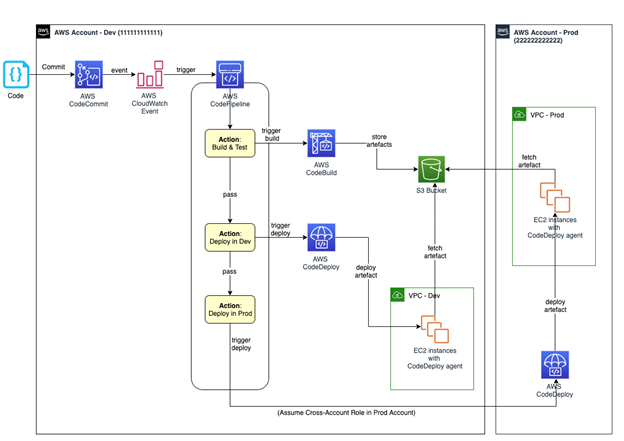
\includegraphics[width=\textwidth]{images/saiful/aws_cicd.png}
    \caption{Workflow of CI/CD pipeline in AWS.}
    \label{fig:aws_cicd}
\end{figure}

%

\subsubsection{Estimated Cost}
%
Amazon follows a 'pay as you go model to charge its clients. A user only needs to pay when he uses any of the resources or services. Additionally, many of the services offer some basic free trials, which are very useful for testing simple applications. Though, we can say the pricing structure can be a bit complicated for complex applications using various AWS services.\cite{AWS_Cost} The cost can be calculated based on the usage and configuration of the CI/CD pipeline and other resources using the AWS Pricing Calculator (https://calculator.aws/). With the basic configuration of the resources and services mentioned in the previous section, an estimated \$15 per month bill can be expected.\footnote{https://aws.amazon.com/getting-started/projects/set-up-ci-cd-pipeline/services-costs/}
%

\subsubsection{Advantages}
%
AWS is a fast-growing cloud provider for its several advantages. Both individuals and organizations are moving into AWS services for its simplicity, flexible pricing plans, and other facilities. AWS provides a user-friendly UI, which makes it very simple to use for new users. It also provides state-of-the-art security and reliability for all of its resources. The Auto Scaling service automatically adjusts the capacity of the resources. The scalability and elasticity include both downscaling and upsizing. With the pay-as-you-go pricing structure, the users have to pay less and only for the duration of usage. With the rapidly growing network of AWS over the world, the scope of operation is also expanding with more availability. AWS is offering more and more services targeting the needs of the users.



%


\subsubsection{Disadvantages}
As everything has its limitations, Amazon Web Services comes with a few disadvantages. Some may find it difficult to calculate the overall cost for a large company using numerous AWS services. An essential fact for keeping the cost minimum is to utilize the resources efficiently. Additional charges may be applied for technical supports, which differs for different consumer types. There are also some differences between the default limits on the same resources in different regions. AWS offers several similar services that make the users overwhelmed while choosing the right services for their needs.





